\section*{Aufgabe 1}

%Die Simulationen wurden folgende Einstellungen verwendet, sofern nicht anders
%gekennzeichnet:
%\begin{itemize}
%    \item $N = 16$
%    \item $r_\text{c} = \frac{L}{2}$
%    \item $h = \num{0,01}$
%    \item $k_\text{B} = 1$
%    \item $m_\text{i} = 1 \quad \forall i = 1, ..., N$
%    \item Anzahl Freiheitsgrade $N_\text{f} = 2 N - 2$
%\end{itemize}
%Längen werden zudem in Einheiten von $\sigma$ und Zeiten in Einheiten von $\tau$ gemessen.
%Energien und $k_\text{B} T$ werden in Einheiten von $\varepsilon$ gemessen.

\subsection*{a) Initialisierung}

Zu Beginn werden die Orte und Geschwindigkeiten der Teilchen in einer $[0,L] \cdot [0,L]$ Box initialisiert.
Dabei werden zufällige Startgeschwindigkeiten im Bereich \([0, 10]\) gewählt. 
Zusätzlich wird die Schwerpunktsbewegung der Teilchen auf Null gesetzt.
Um die Geschwindigkeiten entsprechend der Temperatur umskalieren zu können, wird folgende Rechnung betrachtet:
\begin{align*}
    T_0 &=
    \frac{2}{k_\text{B} N_\text{f}} \sum_{i=1}^N \frac{\vec{p}_\text{i}^2}{2 m_\text{i}} \\
    &= \frac{1}{N_\text{f}} \sum_{i=1}^N \left(v_\text{x}^2 + v_\text{y}^2\right) \\
    &= \frac{1}{N_\text{f}} \sum_{i=1}^N
        \left(a^2 \tilde{v}_\text{x}^2 + a^2 \tilde{v}_\text{y}^2\right) \\
    &= a^2 \frac{1}{N_\text{f}} \sum_{i=1}^N
        \left(\tilde{v}_\text{x}^2 + \tilde{v}_\text{y}^2\right) \\
    &= a^2 \tilde{T}.
\end{align*}
Aus ihr folgt, dass die Geschwindigkeiten mit 
\begin{equation*}
    \frac{1}{a} = \sqrt{\!\left(\frac{\tilde{T}}{T}\right)}
\end{equation*}
skaliert werden müssen.

\FloatBarrier
\subsection*{b) Äquilibrierung}

Die Dynamik des Systems wird nun mithilfe des Geschwindigkeits-Verlet-Algorithmus ermittelt.
Die dabei benötigte Beschleunigung der einzelnen Teilchen ergibt sich aufgrund normierter Massen von 1
direkt aus der Kraft, welches sich wiederum aus dem Lennard-Jones Potential
\begin{align*}
    \vec{F}_\text{i}
    &= \sum_{i \neq j} \vec{F}_\text{ij}
    = - \sum_{i \neq j} \sum_{\vec{n} \in \mathbb{Z}^2}
        \frac{\vec{r}_\text{ij} + L \vec{n}}{\left|\vec{r}_\text{ij} + L \vec{n}\right|}
        V'\left(\left|\vec{r}_\text{ij} + L \vec{n}\right|\right) \\
    \text{Cutoff } r_\text{c}
    &= \frac{1}{2} L < \left|\vec{r}_\text{ij} + L \vec{n}\right| \\
    \vec{F}\!\left(\vec{r}\right)
    &= - \vec{\nabla} V\left(r\right)
    = - 24 \frac{\vec{r}}{r^2}
        \left[2 \left(\frac{1}{r}\right)^{-12} - \left(\frac{1}{r}\right)^{-6}\right]
\end{align*}
ergibt.
Dabei stellt der Cutoff $r_\text{c}$ sicher, dass ein Teilchen $i$ nur einmal mit einem (Bild)Teilchen $j$
wechselwirkt.

Die während der Äquilibrierung ergeben sich die Schwerpunktsgeschwindigkeit $\vec{v}_\text{S}$,
die Temperatur $T$, die potentielle und die kinetische Energie
($E_\text{pot}$, $E_\text{kin}$) mithilfe von
\begin{align*}
    \vec{v}_\text{S} &= \frac{1}{N} \sum_{i=1}^N \vec{v}_\text{i} \\
    E_\text{pot} &= \sum_{i=1}^N \sum_{j=i+1}^N
        V\!\left(\left|\vec{r}_\text{i} - \vec{r}_\text{j}\right|\right) \\
    E_\text{kin} &= \sum_{i=1}^N \frac{1}{2} \vec{v}_\text{i} \\
    T &= \frac{2}{N_\text{f}} E_\text{kin}
\end{align*}
berechnet.

Diese genannten größen werden in Abbildung \ref{fig:T1}, \ref{fig:v1} und \ref{fig:e1}
dargestellt. Da sich die Temperatur aus der kinetischen Energie berechnet, zeigen sie
denselben Verlauf.

\begin{figure}
    \centering
    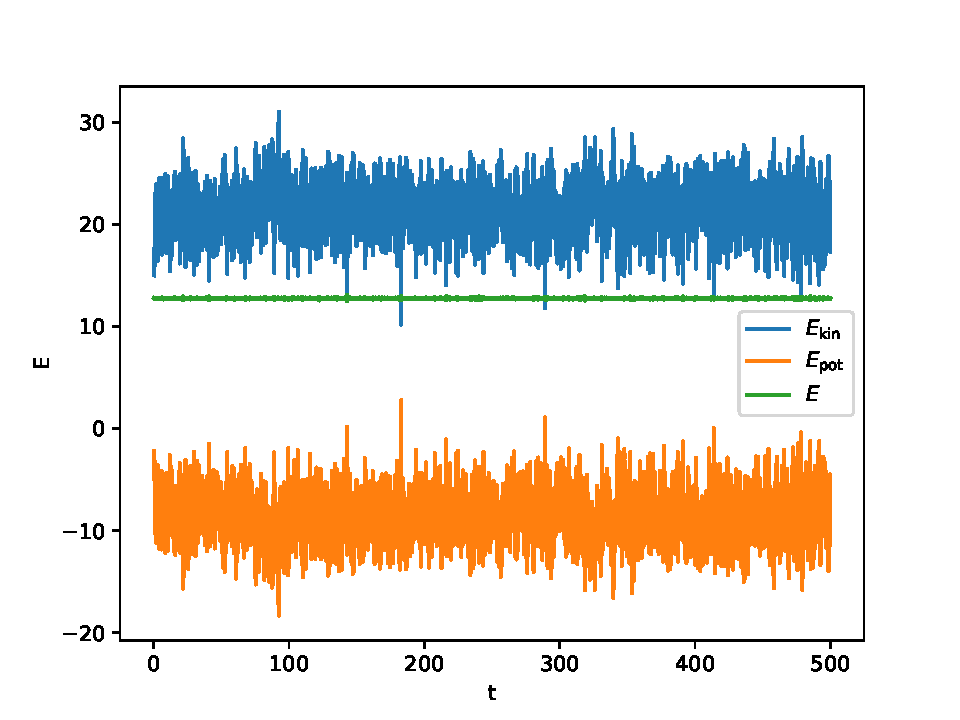
\includegraphics[width=0.45\textwidth]{A1/build/aequi1_E.pdf}
    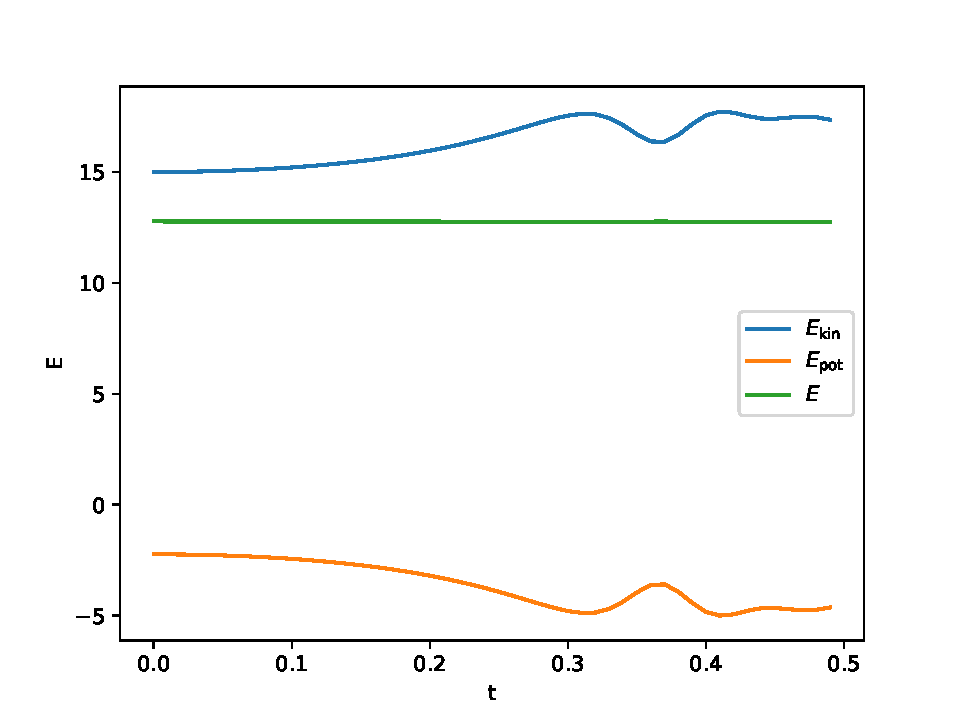
\includegraphics[width=0.45\textwidth]{A1/build/aequi1_EE.pdf}
    \caption{ $T_0 = 1\:\varepsilon$.}
    \label{fig:e1}
\end{figure}

\begin{figure}
    \centering
    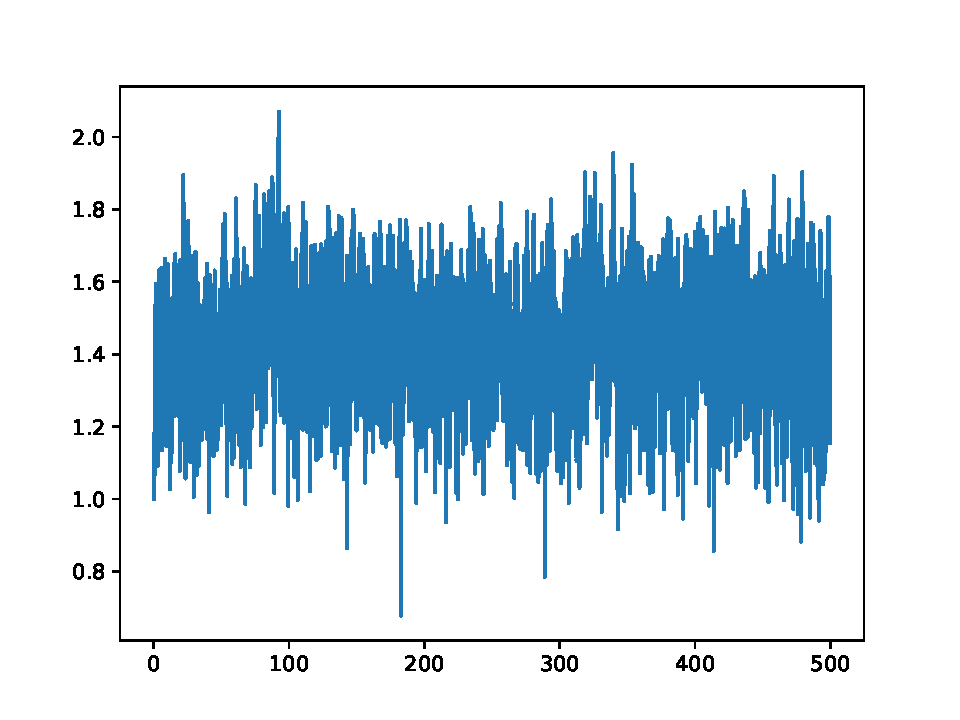
\includegraphics[width=0.45\textwidth]{A1/build/aequi1_T.pdf}
    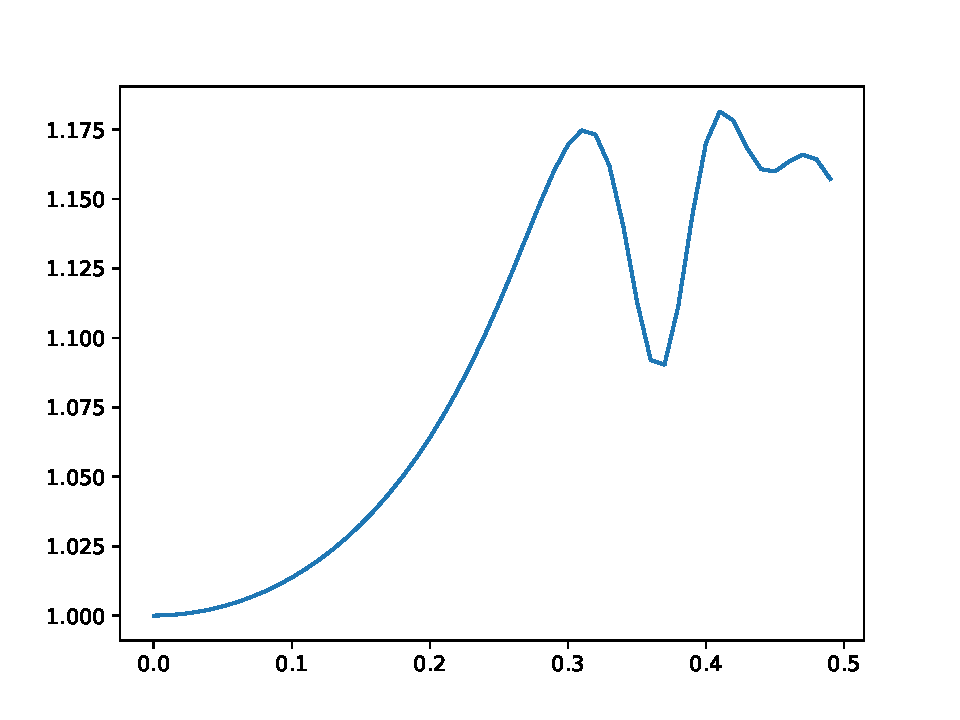
\includegraphics[width=0.45\textwidth]{A1/build/aequi1_TT.pdf}
    \caption{$T_\text{0} = 1\:\varepsilon$.}
    \label{fig:T1}
\end{figure}

\num{1e-15}.
\begin{figure}
    \centering
    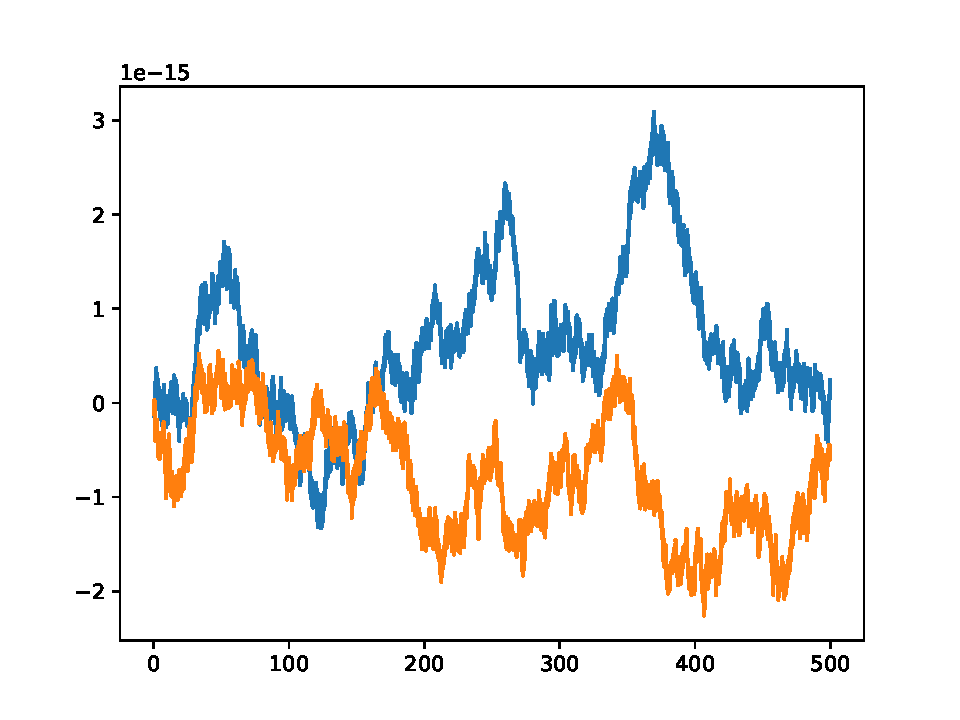
\includegraphics[width=0.45\textwidth]{A1/build/aequi1_V.pdf}
    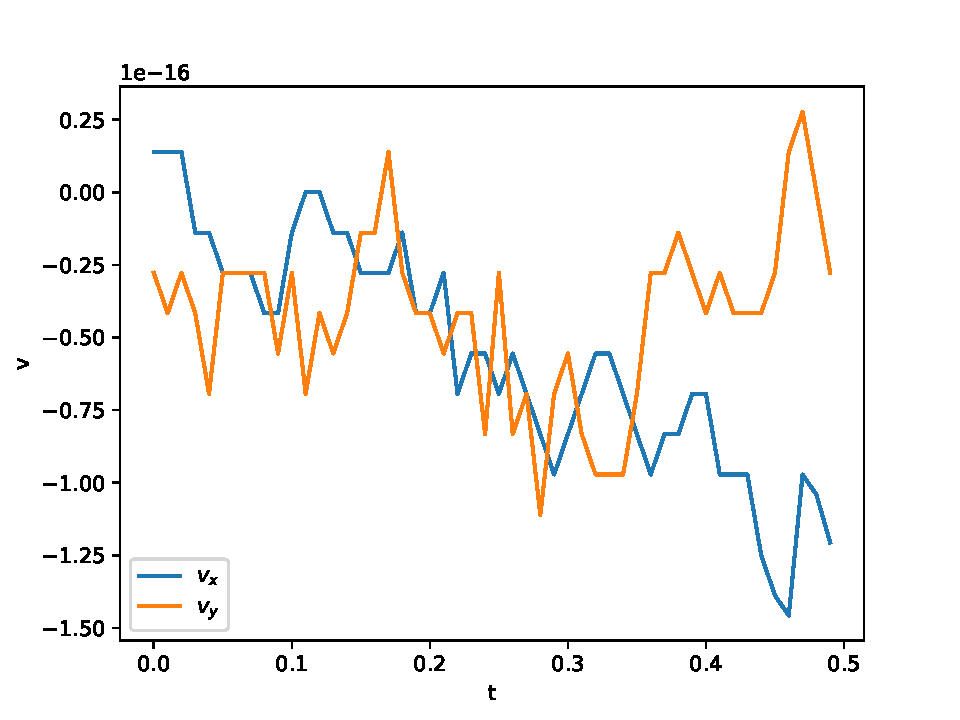
\includegraphics[width=0.45\textwidth]{A1/build/aequi1_VV.pdf}
    \caption{$T_\text{0} = 1\:\varepsilon$.}
    \label{fig:v1}
\end{figure} 

\FloatBarrier
\subsection*{c) Messung}
Die Mittelung der Temperaturen für $5\cdot 10^5$ Schritten ergibt für die jeweiligen Temperaturen:

\begin{align}
    \text{ T1:  } &  1.4791  \pm  0.1287 \\
    \text{ T2:  } &  0.6993  \pm  0.1206 \\
    \text{ T3:  } & 96.3769  \pm  4.6857 \\
\end{align}
In den Abbildungen \ref{fig:messung_T=1_temp} bis \ref{fig:messung_T=1e-2_temp}
sind die zeitlichen Verläufe der Temperatur
bei verschiedenen Starttemperaturen dargestellt.

\begin{figure}
    \centering
    \includegraphics[height=8cm]{build/messung_T1_temp.jpg}
    \caption{Temperaturverlauf der Messung bei $T_\text{init} = 1\:\varepsilon$.}
    \label{fig:messung_T=1_temp}
\end{figure}
\begin{figure}
    \centering
    \includegraphics[height=8cm]{build/messung_T1e2_temp.jpg}
    \caption{Temperaturverlauf der Messung bei $T_\text{init} = 100\:\varepsilon$.}
    \label{fig:messung_T=1e2_temp}
\end{figure}
\begin{figure}
    \centering
    \includegraphics[height=8cm]{build/messung_T1e-2_temp.jpg}
    \caption{Temperaturverlauf der Messung bei $T_\text{init} = 0.01\:\varepsilon$.}
    \label{fig:messung_T=1e-2_temp}
\end{figure}


\FloatBarrier
 \subsection*{d) Thermostat}

Für den Fall, dass ein isokinetisches Thermostat verwendet wird, werden nach jedem Schritt die Geschwindigkeiten so skaliert, dass das System wieder die Ursprungstemperatur gehalten wird.
Der Verlauf der Energien während der Äquilibrierungsphase für $T_\text{init} = 0.01$ ist in Abbildung \ref{fig:thermostat_equi_energy}   dargestellt.

Da die Temperatur recht klein gewählt ist, bewegen sich die Teilchen nicht viel
und sollten eine periodische Anordnung einnehmen.
In Abbildung \ref{fig:endkonfig} ist die Konfiguration nach der Messung dargestellt.
Es zeigt sich, dass kleinere Muster erkennbar sind.
Dies spricht für eine feste Phase der Teilchen.
\begin{figure}
    \centering
    \includegraphics[height=8cm]{build/thermostat_equi_energy.jpg}
    \caption{Energieverlauf während der Äquilibrierungsphase bei isokinetischem Thermostat.}
    \label{fig:thermostat_equi_energy}
\end{figure}
\begin{figure}
    \centering
    \includegraphics[height=6cm]{build/endkonfig.jpg}
    \caption{Endkonfiguration mit 16 Teilchen bei isokinetischem Thermostat.}
    \label{fig:endkonfig}
\end{figure}
